% Options for packages loaded elsewhere
\PassOptionsToPackage{unicode}{hyperref}
\PassOptionsToPackage{hyphens}{url}
%
\documentclass[
]{article}
\usepackage{amsmath,amssymb}
\usepackage{lmodern}
\usepackage{iftex}
\ifPDFTeX
  \usepackage[T1]{fontenc}
  \usepackage[utf8]{inputenc}
  \usepackage{textcomp} % provide euro and other symbols
\else % if luatex or xetex
  \usepackage{unicode-math}
  \defaultfontfeatures{Scale=MatchLowercase}
  \defaultfontfeatures[\rmfamily]{Ligatures=TeX,Scale=1}
\fi
% Use upquote if available, for straight quotes in verbatim environments
\IfFileExists{upquote.sty}{\usepackage{upquote}}{}
\IfFileExists{microtype.sty}{% use microtype if available
  \usepackage[]{microtype}
  \UseMicrotypeSet[protrusion]{basicmath} % disable protrusion for tt fonts
}{}
\makeatletter
\@ifundefined{KOMAClassName}{% if non-KOMA class
  \IfFileExists{parskip.sty}{%
    \usepackage{parskip}
  }{% else
    \setlength{\parindent}{0pt}
    \setlength{\parskip}{6pt plus 2pt minus 1pt}}
}{% if KOMA class
  \KOMAoptions{parskip=half}}
\makeatother
\usepackage{xcolor}
\usepackage[margin=1in]{geometry}
\usepackage{longtable,booktabs,array}
\usepackage{calc} % for calculating minipage widths
% Correct order of tables after \paragraph or \subparagraph
\usepackage{etoolbox}
\makeatletter
\patchcmd\longtable{\par}{\if@noskipsec\mbox{}\fi\par}{}{}
\makeatother
% Allow footnotes in longtable head/foot
\IfFileExists{footnotehyper.sty}{\usepackage{footnotehyper}}{\usepackage{footnote}}
\makesavenoteenv{longtable}
\usepackage{graphicx}
\makeatletter
\def\maxwidth{\ifdim\Gin@nat@width>\linewidth\linewidth\else\Gin@nat@width\fi}
\def\maxheight{\ifdim\Gin@nat@height>\textheight\textheight\else\Gin@nat@height\fi}
\makeatother
% Scale images if necessary, so that they will not overflow the page
% margins by default, and it is still possible to overwrite the defaults
% using explicit options in \includegraphics[width, height, ...]{}
\setkeys{Gin}{width=\maxwidth,height=\maxheight,keepaspectratio}
% Set default figure placement to htbp
\makeatletter
\def\fps@figure{htbp}
\makeatother
\setlength{\emergencystretch}{3em} % prevent overfull lines
\providecommand{\tightlist}{%
  \setlength{\itemsep}{0pt}\setlength{\parskip}{0pt}}
\setcounter{secnumdepth}{5}
\ifLuaTeX
  \usepackage{selnolig}  % disable illegal ligatures
\fi
\IfFileExists{bookmark.sty}{\usepackage{bookmark}}{\usepackage{hyperref}}
\IfFileExists{xurl.sty}{\usepackage{xurl}}{} % add URL line breaks if available
\urlstyle{same} % disable monospaced font for URLs
\hypersetup{
  pdftitle={Resolução do livro `Mecánica: Berkeley Physics Course - Vol 1'},
  pdfauthor={Igo da Costa Andrade},
  hidelinks,
  pdfcreator={LaTeX via pandoc}}

\title{Resolução do livro `Mecánica: Berkeley Physics Course - Vol 1'}
\author{Igo da Costa Andrade}
\date{2023-05-31}

\begin{document}
\maketitle

{
\setcounter{tocdepth}{2}
\tableofcontents
}
\hypertarget{resoluuxe7uxe3o-de-problemas}{%
\section*{Resolução de Problemas}\label{resoluuxe7uxe3o-de-problemas}}
\addcontentsline{toc}{section}{Resolução de Problemas}

KITTEL, C.; KNIGHT, W. D.; MALVIN, A. R. \textbf{Mecánica}: Berkeley Physics Course. v. 1. 2. ed.~Barcelona: Reverté, 1989.

\begin{figure}
\centering
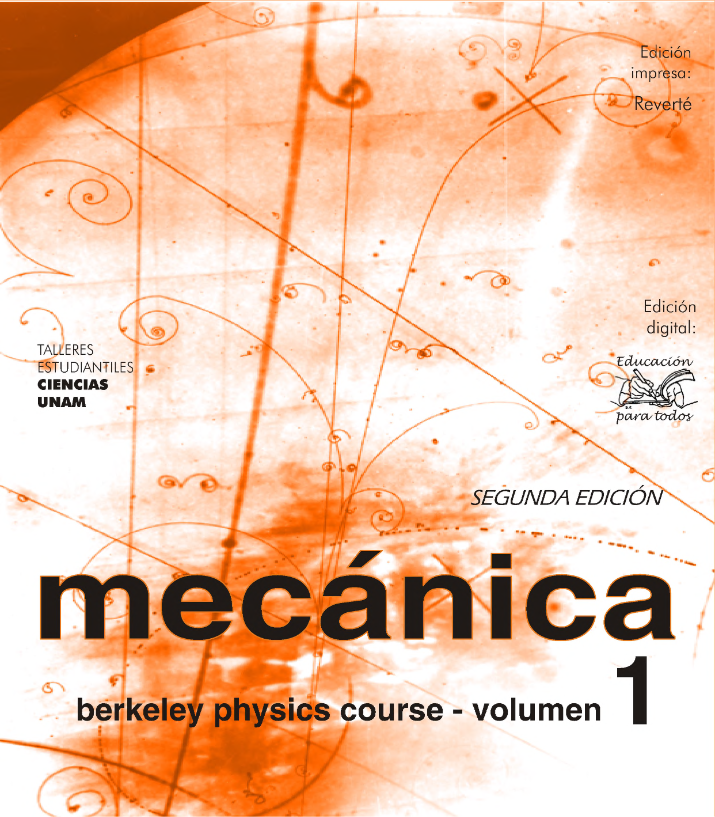
\includegraphics{img/berkeley_vol_1_cover.png}
\caption{Capa do livro Curso de Física de Berkeley - Vol 1 - Mecánica}
\end{figure}

\hypertarget{introduuxe7uxe3o}{%
\section{Introdução}\label{introduuxe7uxe3o}}

\hypertarget{problemas}{%
\subsection*{Problemas}\label{problemas}}
\addcontentsline{toc}{subsection}{Problemas}

\begin{enumerate}
\def\labelenumi{\arabic{enumi}.}
\tightlist
\item
  \emph{O Universo conhecido}. Utilizando a informação dada no texto, estimar as seguintes magnitudes:
\end{enumerate}

\begin{enumerate}
\def\labelenumi{\alph{enumi}.}
\item
  A massa total do Universo conhecido.

  \textbf{Resp.:}
  \begin{align*}
     &x = \dfrac{-b \pm \sqrt{b^2 - 4ac}}{2a}\\
     &x = -2
   \end{align*}
\item
  A densidade média da matéria no Universo.
\item
  A relação entre o raio do universo conhecido e o do próton. (Tomar o raio do próton como \(10^{-13}\) cm; massa do próton: \(1,7 \times 10^{-29}\) g.)
\end{enumerate}

\begin{enumerate}
\def\labelenumi{\arabic{enumi}.}
\setcounter{enumi}{1}
\tightlist
\item
  \emph{Sinais que atravessam um próton}.
\end{enumerate}

\hypertarget{vetores}{%
\section{Vetores}\label{vetores}}

\end{document}
